\documentclass[12pt,a4paper,openright,twoside]{book}
\usepackage[utf8]{inputenc}
\usepackage{disi-thesis}
\usepackage{code-lstlistings}
\usepackage{notes}
\usepackage{shortcuts}
\usepackage{acronym}
\usepackage{subfig}
\usepackage[inline]{enumitem}


\school{\unibo}
\programme{Corso di Laurea Magistrale in Ingegneria e Scienze Informatiche}
% \title{Addressing Fairness in \ac{AI} Systems:\newline a Pragmatic (Meta-)Methodology and its Reification into a Software System}
\title{Addressing Fairness in \acs{AI} Systems: Design and Development of a Pragmatic (Meta-)Methodology}
% \title{Addressing Fairness in \ac{AI} Systems: a Pragmatic (Meta-)Methodology from an Engineering Perspective}
\author{Mattia Matteini}
\date{\today}
\subject{Intelligent Systems Engineering}
\supervisor{Prof.\ Giovanni Ciatto}
\cosupervisor{Prof.\ Roberta Calegari}
\morecosupervisor{Prof.\ Andrea Omicini}

\session{IV}
\academicyear{2023--2024}

% Definition of acronyms
\acrodef{AI}{Artificial Intelligence}
\acrodef{BU}{Business User}
\acrodef{TU}{Technical User}
\acrodef{Q/A}{Question--Answering}
\acrodef{DDD}{Domain Driven Design}
\acrodef{API}{Application Programming Interface}

% temporary fix for acronyms (https://github.com/oetiker/acronym/issues/62)
\makeatletter
\AtBeginDocument
 {
   \def\ltx@label#1{\cref@label{#1}}%add braces
   \def\label@in@display@noarg#1{\cref@old@label@in@display{#1}}%remove braces  
 } %
\makeatother

\mainlinespacing{1.241} % line spacing in mainmatter, comment to default (1)

\begin{document}

\frontmatter\frontispiece

\begin{abstract}	
Max 2000 characters, strict.
\end{abstract}


\begin{dedication} % this is optional
Optional. Max a few lines.
\end{dedication}

%----------------------------------------------------------------------------------------
\tableofcontents   
\listoffigures     % (optional) comment if empty
\lstlistoflistings % (optional) comment if empty
%----------------------------------------------------------------------------------------

\mainmatter

%----------------------------------------------------------------------------------------
\chapter{Introduction}%
\label{chap:introduction}
%----------------------------------------------------------------------------------------


\paragraph{Structure of the Thesis}

\note{At the end, describe the structure of the paper}




%----------------------------------------------------------------------------------------
\chapter{Background}%
\label{chap:background}
%----------------------------------------------------------------------------------------

\section{What is Fairness?}
%
% 1. explaining what is normal fairness, from an ethical and social perspective
%
Fairness, from an ethical and social perspective, is the principle of treating individuals and groups equitably, ensuring that no one is unjustly advantaged or disadvantaged due to biases, discrimination, or arbitrary distinctions.
%
It is deeply rooted in moral philosophy, legal systems, and societal norms, aiming to promote justice, equality, and inclusion.
%
A just society requires reducing social inequalities, and ensuring that opportunities and resources are distributed in a way that acknowledges both individual merit and systemic disadvantages.
%
The concept of fairness evolves based on cultural, historical, and contextual factors, reflecting a society’s commitment to ethical treatment and social cohesion.


\paragraph{Fairness in \acs{AI}.}

% 2. explaining what is fairness in AI, from a technical perspective
From a technical point of view, fairness in \ac{AI} refers to the development and deployment of \ac{AI} systems that minimize biases and prevent discriminatory outcomes.
%
It involves designing systems that ensure equitable treatment across different demographic groups, particularly those historically marginalized or disadvantaged.
%
% Fairness in AI can be assessed using various mathematical definitions, such as demographic parity, equalized odds, and fairness through unawareness, depending on the context and application.
%
The main challenges in this field are building \texttt{fair-by-design} systems, namely such systems in which the fairness problem is addressed since the very beginning of the process, and detecting biases in already existing systems, mitigating them if possible.
%
% The challenge in AI fairness lies in defining and balancing these technical fairness measures while maintaining model accuracy and practical utility.

Before the advent of fairness, \ac{AI} systems were developed with the primary goal of optimizing performance metrics, such as accuracy.
%
Nowadays, that fairness is becoming a crucial aspect to consider, accuracy is no more the only metric to optimize, it is necessary to find a balance between accuracy and fairness.
%
Besides that, fairness can also be in contrast with the performance of the model, making difficult to find a good trade-off between these two aspects.

% 3. explaining why fairness in AI is important
Fairness is becoming crucial because \ac{AI} systems increasingly influence decision-making processes in various sectors of society, including hiring, lending and healthcare.
%
If \ac{AI} models are biased, they can perpetuate and even amplify existing societal inequalities, leading to unjust outcomes and tremendous effects on individuals and communities.
%
Ensuring fairness in \ac{AI} enhances trust, transparency, and accountability, making \ac{AI} systems more ethical, reliable, and beneficial for society.

% 3.1 speaking about some history of AI and the fact is getting more and more important and utilized in many fields
\ac{AI} has undergone significant advancements over the past few decades, causing an enormous increase in its adoption across various domains, until becoming pervasive in the daily life of people.
%
This also caused a growing of biases in \ac{AI} systems, as discriminations are intrinsically part of the human history, and consequently of the data that \ac{AI} systems are trained on.


% 3.2 speaking about the fact that AI is used in many critical fields, and the fact that fairness is important in these fields

\ac{AI} is now widely used in critical domains such as healthcare, finance, education, and criminal justice, where biased decisions can have life-altering consequences.
%
For instance, in healthcare, biased algorithms may lead to misdiagnosis or unequal treatment recommendations for different demographic groups;
%
in finance, \ac{AI}-driven credit scoring models can reinforce discriminatory lending practices, limiting access to financial resources;
%
in the criminal justice system, biased predictive policing and risk assessment tools can disproportionately target marginalized communities.
%
Given these risks, ensuring fairness in \ac{AI} is essential to preventing discrimination, maintaining ethical standards, and safeguarding individuals.


\paragraph{On Multidisciplinarity.}

% 4. AI fairness is a multidisciplinary concept.

Achieving fairness in \ac{AI} requires a multidisciplinary approach that integrates insights from computer science, ethics, law and social sciences.
%
Technical methods alone cannot fully address fairness, as fairness is deeply tied to societal values, human rights, and legal frameworks.
%
Socio-legal experts help define fairness principles, ensure compliance with anti-discrimination laws and analyze the societal impact.
%
The intersection of these fields highlights that \ac{AI} fairness is not merely a technical challenge but a complex, multidimensional issue requiring collective effort and interdisciplinary research and collaboration.

% 4.1 explaining the link with the socio-legal perspective and contraints, citing AI Act

An impactful example regarding the work of legal experts in the field of \acl{AI} is the \textit{AI Act}~\cite{madiega2021artificial}.
%
The AI Act, proposed by the European Union, is a comprehensive regulatory framework designed to ensure that AI systems are safe, transparent, and aligned with fundamental rights.
%
It categorizes AI applications into different risk levels—unacceptable risk, high risk, limited risk, and minimal risk—imposing stricter requirements on higher-risk systems, such as those used in hiring, law enforcement, and healthcare.
%
These requirements include transparency, human oversight, and bias mitigation.
%
However, translating these legal constraints into practical technical steps is not trivial.

Concepts like fairness, accountability, and explainability are difficult to quantify, and AI models often operate as black boxes, making compliance complex.
%
While the AI Act sets an important precedent for AI governance, its effective implementation requires further collaboration between policymakers, legal experts, and computer scientist to bridge the gap between regulation and technical feasibility.


\paragraph{Measuring Fairness.}
% 5. How to assess and measure fairness?

At one point, in order to assess the fairness of an \ac{AI} system, is important to have a way to ``measure'' how much the system is fair and in what terms.
%
Remarking what said before, fairness is very context-dependent, and there is not a single way to measure it. 

% 5.1 define fairness metrics

The need to cover multiple aspects of fairness has led to the introduction of various \textit{fairness metrics}---statistical formulas that quantify fairness in different ways, each capturing a slightly different aspect of fairness.
%
These fairness metrics, are a set of indexes that can be used to detect biases in \ac{AI} systems, and they can be used indeed to evaluate the fairness of a model.
%

% 5.2 list the main fariness matrics providing a brief description and formal definition

In the following, are listed some of the most common fairness metrics used in the literature~\cite{DBLP:conf/bias/IrfanML23}:

\begin{itemize}
    \item \textit{Statistical Parity Difference} (SPD) measures the difference between the probability of the privileged and unprivileged classes receiving a favorable outcome. This measure should be equal to 0 to be fair.
    
    Formally it is defined as $SPD = P(\hat{Y} = 1 | A = a) - P(\hat{Y} = 1 | A = b)$
    %
    where $A$ is the sensitive attribute, $\hat{Y}$ is the predicted outcome, and $a$ and $b$ are the privileged and unprivileged groups, respectively.
    
    \item \textit{Disparate Impact} (DI) compares the proportion of individuals that receive a favorable outcome for two groups, a privileged group and an unprivileged group. This measure should be equal to 1 to be fair.
    
    Formally it is defined as $DI = P(\hat{Y} = 1 | A = a) / P(\hat{Y} = 1 | A = b)$
    %
    where $A$ is the sensitive attribute, $\hat{Y}$ is the predicted outcome, and $a$ and $b$ are the privileged and unprivileged groups, respectively.
    \sidenote{add more metrics?}
    
\end{itemize}


\note{manca una sezione Lack of engineering methodology?}


\section{\acs{AI} Lifecycle}

% 1. AI lifecycle changes a lot if we consider fairness, speak about lifecycle in general, and speak about the changes that fairness introduces

Since the very beginning of the \ac{AI} era, the standard lifecycle consists of the following ``traditional'' steps:
\begin{enumerate*}[label= (\roman*)]
    \item data collection and processing,
    \item model training,
    \item system evaluation.
\end{enumerate*}
%
Obviously, this workflow in the latest years have increased in complexity and now, with the newer innovations and powerful models and architectures, it may appear even almost minimalistic, but it still represents the core of all \ac{AI} systems.

However, when fairness is taken into account, each step needs to be revisited in order to obtain an equitable, impartial, and fair \ac{AI} system.

% 2 fairness can be achieved only if socio-legal perspective is taken into account, talk about the importance of the socio-legal perspective

To achieve this goal, the technical perspective is not enough.
%
Fairness is a multidisciplinary concept that involves social, legal, and ethical aspects.
%
Therefore, the \ac{AI} lifecycle needs to be constrained by socio-legal requirements that engineers must consider during the development process.
%
This includes understanding the societal impact of \ac{AI} systems, ensuring compliance with legal standards, and adhering to ethical guidelines.

There are also many differences between the socio-legal and technical perspectives.
%
Regarding the \ac{AI} lifecycle, engineers tend to focus on technical aspects and few development phases, in fact the major part of the literature speaks only about \textit{pre-processing}, \textit{in-processing} and \textit{post-processing} (\Cref{fig:ai-lifecycle}).
%
\begin{figure}
    \centering
    \includegraphics[width=.6\linewidth]{figures/ai-lifecycle.png}
    \caption{Fair \acs{AI} lifecycle from~\cite{DBLP:conf/ijcai/CalegariCMO23}}
    \label{fig:ai-lifecycle}
\end{figure}
%
Respectively, \textit{pre-processing} involves data collection and preparation, \textit{in-processing} refers to the model training phase, and \textit{post-processing} deals with the fair evaluation of the \ac{AI} system.

Often engineers adopt reductionist approaches addressing a field that is not their own, discarding the big picture of social, economic, and institutional constraints.
%
On the other hand, socio-legal experts consider a broader range of activities and phases.
%
They focus on ``building blocks'' for fair \ac{AI} such as risk assessment, stakeholder identification, regulatory analysis, and fundamental human rights impact assessment.
%
In particular, with respect to fundamental rights impact assessments, these will be legally required for some \ac{AI} systems, yet no standard for implementing them has emerged so far.




\section{Practical Issues}

\subsection{What is (un)fair?}

% 1. the notion of fairness is subjective 

Fairness in \ac{AI} (and beyond) is inherently subjective, shaped by cultural values, ethical theories, and individual perspectives.
%
What one group considers fair may not align with other people’s understanding, leading to debates about determining what is fair and what is not.
%
This subjectivity and variation in viewpoints complicates efforts to develop standardized fairness metrics, as no single approach can universally capture the diverse and often conflicting notions of fairness present across different social, legal, and institutional contexts.

% 2. the notion of fairness is also context-dependent 

Beyond its subjectivity, fairness is also highly context-dependent. The same algorithm might be considered fair in one application but biased in another, depending on the societal, legal, and institutional constraints surrounding it.
%
For instance, fairness considerations in hiring algorithms differ from those in criminal justice risk assessments, necessitating tailored approaches rather than generic solutions.
%
Moving forward, privileged and unprivileged groups change depending on the application domain, as well as the fairness criteria that are taken into account.

\subsection{Bridging Perspectives}
% 3. bridging socio-legal perspective and technical perspective is difficult 

Bridging the socio-legal and technical perspectives on fairness is a significant challenge. 
%
Guidelines and descriptive methodologies exist to address fairness compliance from a social-legal perspective, but their approach offer broad guidelines without defining practical steps, leaving interpretation to technical experts~\cite{hicssfairness2025}.
%
The lack of alignment between these viewpoints makes it difficult to translate abstract fairness principles into concrete computational methods.
%
This also leads to a proliferation of metrics, each measuring slightly different aspects of fairness, reflecting the diverse priorities and domain perspectives.

% 4. socio-legal and technical perspectives speak different languages, 

A fundamental obstacle to this integration is the differing language used by socio-legal experts and technical people.
%
It is difficult to reach an agreement if even a concept or term can assume different meanings depending on the perspective.
% Legal and ethical frameworks rely on qualitative reasoning and precedent, whereas technical disciplines typically speaks about quantitative metrics
This linguistic division creates a difficult barrier to interdisciplinary collaboration, leading to misunderstandings even when working towards shared goals.


% 5. socio-legal and technical perspectives have different backgrounds

These perspectives are shaped also by distinct academic and methodological backgrounds.
%
Legal and ethical frameworks tend to be verbose and highly context-specific, relying on various interpretations and case-by-case analyses.
%
In contrast, technical disciplines prioritize concrete steps and pragmatic aspects.

% 6. lack of methodology that takes into account both perspectives

In literature, there is a lack of methodologies regarding the building of fair \ac{AI} systems.
%
The lack is not just related to the technical perspective, but also to the socio-legal one.
%
This is enhanced by the fact that design and develop a single methodology fitting all kinds of \ac{AI} systems is not feasible, as the system requirements and constraints change depending on the context and the application domain.
%
Of course, the creation of such methodology is damaged by the multidisciplinary complexity of the problem, and should involve expertises across all the relevant fields.


% % ----------------


% You may also put some code snippet (which is NOT float by default), eg: \cref{lst:random-code}.

% \lstinputlisting[float,language=Java,label={lst:random-code}]{listings/HelloWorld.java}


%----------------------------------------------------------------------------------------
\chapter{The Meta-Methodology}%
\label{chap:meta-methodology}
%----------------------------------------------------------------------------------------

% 0. explaining what is a methodology and why we need it to build fair AI systems

A \textbf{methodology} is a structured framework that outlines the principles, processes, techniques and best practices used to conduct research or develop systems in a systematic and reproducible manner.
%
In this context, a well-defined methodology would be essential for ensuring fairness, as it would provide a rigorous approach to
\begin{enumerate*}[label=(\roman*)]
    \item translating socio-legal requirements into technical steps,
    \item identifying and mitigating biases, and
    \item building \texttt{fair-by-design} systems.
\end{enumerate*}
\sidenote{need to introduce the concept of \texttt{fair-by-design} systems in Background chapter}

Having a rigorous methodology would impact the development of fair \ac{AI} systems, it means that it would represent a clear way to follow, encapsulating the already existing unclear guidelines provided by the socio-legal frameworks.

% x why META-methodology
Unfortunately, factors such as multidisciplinarity, complexity, and context-dependency make it difficult to design a single methodology that fits all contexts and applications.
%
Therefore, this contribution proposes a \textbf{meta-methodology} that provides a flexible and adaptable framework for design and develop multiple methodologies instead of a single one.
%
The idea of the meta-methodology comes from the sessions of brainstorming and discussions between experts of different fields, where troubles are emerged in reaching an agreement and proceeding with clear technical steps relying on the legal requirements.

% The meta-methodology consists of the following key components:

\section{Desiderata}
In the following, are listed the desiderata that the meta-methodology should satisfy.
% 1. List the meta-methodology desiderata/requirements


\begin{enumerate}[label=\textbf{R\arabic*}, ref=R\arabic*]
    
    % 1.1 the methodology should assist experts in translating the social-legal requirements into practice
    \item\label{req:R1} \textbf{Requirements Translation}: The methodology should assist experts in translating the socio-legal requirements into practice.

    A big challenge in this field, is to understand how legal constraints can be applied, and how technical steps can be identified to satisfy the requirements. That's why the methodology should provide a mechanism assisting this phase.
    
    % 1.2 the methodology should consider the cultural context and the domain AI system under design
    \item\label{req:R2} \textbf{Context and Domain Awareness}: The methodology should consider the cultural context and the domain of \ac{AI} system under design.
    
    AI systems have been applied in several (and critical) use cases. For each of them, the constraints and requirements change, so through the methodology, it should be possible to understand the system domain and be context-aware.

    % 1.3 the methodology should adapt to any change in the cultural context as it evolves
    \item\label{req:R3} \textbf{Adaptability}: The methodology should adapt to any change in the cultural context as it evolves.
    
    Some context could be volatile in terms of societal norms and cultural changes, so the methodology should be able to adjust and align to new constraints.
    
    % 1.4 the methodology should account for both pre-existing AI systems, datasets, and algorithms, and new AI systems
    \item\label{req:R4} \textbf{Legacy and Novel Systems}: The methodology should account for both pre-existing and new \ac{AI} systems.
    
    It is reasonable that the methodology should be able to be applied to new software systems, but it would be a big lack if it could not be applied to already existing systems, remembering that there are a lot of deployed systems that, probably, are not fair.

    % 1.5 the methodology should not just provide a theoretical guideline, but also assist the AI system creation
    \item\label{req:R5} \textbf{Building the AI System}: The methodology should not just provide a theoretical guideline, but also assist the AI system creation. 
    
    This means that it is necessary a software reification of the methodology permitting to be applied practically, obtaining eventually, a fair AI system.
\end{enumerate}


% 2. Concepts
\section{Concepts}

\paragraph{The Roles.}
In the proposed methodology process, there are two main roles involved:
\begin{enumerate}
    \item \textbf{\ac{BU}}, also called \textbf{stakeholder}, who is the person commissioning the \ac{AI} system.
    \item \textbf{\ac{TU}}, who is the person with technical background, assisting the \ac{BU} in the development of the \ac{AI} system.
\end{enumerate}

With respect to \ac{BU}, it is assumed that he or she may have limited or no technical knowledge.
%
This is a common scenario in the real world, where often stakeholders are people with a specific domain expertise, but not necessarily with technical skills.
%
One of the goal of the methodology, is to provide a way to assist the \ac{BU} in the development of the \ac{AI} system, without requiring necessarily deep technical knowledge.
%
Potentially, stakeholder could even build a fair \ac{AI} system without the need of a \ac{TU}.

On the other hand, the \acl{TU}, despite is the person with technical background, is not the responsible for the entire system development.
%
Firstly, \ac{TU} must be able to assist \ac{BU} during the process to clarify any technicalities that may arise, and secondly, he or she must have some knowledge about basics of fairness.

Finally, \ac{TU} may contribute to the system development through the implementation of scripts/computational processes involved in the building of the system and integrated in the methodology.
%
In fact, the software reification of the methodology will be a tool providing \acp{API} for technical people, in order to permit them to attach their scripts.


\paragraph{Questionnaire.}
% 2.1. integration of multiple perspectives and representing legal contraints through a Q/A
Discussions among experts from involved fields highlighted the need for a practical understanding of the domain and the cultural context of the system being designed, ensuring that it is accessible and comprehensible to people of any background.
%
The proposed approach relies on a straightforward questionnaire, which directly engages the \acl{BU} with questions regarding the system's domain.

% 2.1.1 also to represent practical steps
The questionnaire serves as a structured flow of questions and answers designed to gather essential contextual information. Depending on that, it provides practical steps to guide the development of a fair \ac{AI} system.
%
Questionnaire is not just used to collect information, it also acts as a tool to assist the \ac{BU} in making well-informed decisions. At the same time, questions represent also technical steps to be taken, addressing the socio-legal constraints in a comprehensible way.
%
This approach is central to the methodology, owing to its simplicity and versatility in capturing constraints and supporting multiple use cases.
%
The overall concept is shown in \cref{fig:concept}.

\begin{figure}
    \centering
    \includegraphics[width=0.90\linewidth]{figures/concept.pdf}
    \caption{Concept of the proposed approach to fairness engineering from~\cite{hicssfairness2025}.}
    \label{fig:concept}
\end{figure}

% 2.1.2 questions designed ad-hoc from a team of multidisciplinary experts
The pool of questions and answers should be designed ad-hoc from a team of multidisciplinary experts. 
%
This is a crucial, and non-trivial, step in the methodology, as the questions should be able to capture the constraints and requirements from legal frameworks, but also to provide technicalities to be addressed in the proper way and at right time in the process.

Examples of questions that could be asked are:
\begin{itemize}
    \item ``In what area will the \ac{AI} system be applied?'' (Healthcare, Finance, Hiring, etc.)
    \item ``Do you have some AI system already in place, or are you developing an AI system?''
    \item ``Is the dataset sufficiently representative of the population where the system will be used?''
\end{itemize}
%
But also more technical questions like:
\begin{itemize}
    \item ``What are the fairness metrics that should be considered?'' (Statistical Parity Difference, Disparate Impact, etc.)
    \item ``Which are the proxies for the sensitive features?''
    \item ``Which data mitigation algorithm do you want to use?'' (Disparate Impact Remover, Learned Fair Representations, etc.)
\end{itemize}


% 2.2 Order of questions
\paragraph{Order of Questions.}
In the previous paragraph it was mentioned that the flow of questions contains generic and technical questions.
%
The questionnaire should follow a structured approach, beginning with general questions before gradually introducing more technical aspects.
%
Initially, broad and non-technical questions are asked to establish a clear understanding of the system’s domain, purpose, and the cultural or business context in which it operates.
%
As the questionnaire progresses, the questions become more specific and technical.
%
At one point it becomes mandatory to introduce technical aspects because in the end the questionnaire has to converge to the effective building of the fair \ac{AI} system.

% 2.2.1 the order of the questions is important, as the answer to a question can influence the following ones
There is another important concept related to the order of questions: the answer to a question can influence the following ones.
%
This feature is to enable the methodology to adapt to the context and asking later more tailored questions based on the previous answers.
%
Moreover, it is also useful to enrich the part of system development, as it should be possible to follow multiple paths to make an AI system fair.
%
For instance, the \acl{BU} could decide to preprocess the dataset twice, or choose to perform just in-processing mitigation.

These mechanisms lead to a more flexible and adaptable questionnaire, capable of addressing a wide range of contexts and applications, enabling also branching and joining paths in the flow.



% 2.3 Decision support mechanism (emphasis also on stakeholder awareness)
\paragraph{Decision Support.}
% 2.3.1 the Q/A mechanism is also a decision support mechanism
The methodology includes---alongside the \ac{Q/A}---a Decision Support Mechanism, aiming to simplify the process of making decisions regarding fairness-related or complex questions.
%
% 2.3.2 the Q/A mechanism is a way to make the BU aware of the fairness problem
Fairness problem should be taken into account not just by experts in the field, but also by stakeholders, as the relevance of the problem has grown significantly in the last years.
%
% 2.3.3 the Q/A mechanism does not force the BU to make decisions, but it assists him/her in making well-informed decisions
Therefore, an important goal of the methodology is to make the \ac{BU} aware of the fairness problem, and to assist him/her in making well-informed decisions.
%
In this way, the \ac{BU} can gain a deeper understanding of the topic, and can proceed with the development of the system more responsibly.
%
Importantly, the mechanism does not impose decisions but rather suggests the \ac{BU} the answer he or she probably should give.

% 2.3.4 the software also providev additional information and resources to the BU and not just questions
In addition to posing relevant questions and steps, the software provides supplementary information and resources, like charts and tables, helping the \ac{BU} to get a deeper understanding of what he is doing and to assess the fairness of the system more effectively.
\sidenote{in alcuni punti come qui gia parlo di software, prematuro?}


% 3. The Q/A mechanism
\section{The \acs{Q/A} Mechanism}

The \acf{Q/A} mechanism represents the core of this methodology.
%
It has been the starting point to bridge the gap between socio-legal and technical perspectives and provides a structured way to ``translate'' the legal constraints into technical steps, contextualizing them in the application domain.
%
Behind the scenes, the \ac{Q/A} mechanism is a \textbf{directed graph} that represents the decision-making process.

% providing a formal description of the graph
\paragraph{About the Graph.}
Formally, the graph is defined as $G = (V, E)$, where $V$ is the set of nodes and $E$ is the set of directed edges.
%
\textbf{Nodes} consist of two distinct types: \textit{question nodes} and \textit{answer nodes}.
%
Each question node contains a natural language sentence expressing an inquiry, plus an identifier (unique within the whole graph) such as \texttt{Q1}, \texttt{Q2}, etc.
%
They can also contain other arbitrary information, like the type of question (single or multiple choice), a brief description, and so on.
%
Answer nodes, similarly, contain a natural language sentence expressing a possible answer to a question, an identifier (unique within the whole graph) such as \texttt{Q1-A1}, \texttt{Q1-A2}, etc., and other arbitrary and useful information.

\textbf{Edges} are of two sorts too: either \textit{question-to-answer} edges, denoted by $Q \to A$, or \textit{answer-to-question} edges, denoted by $A \to Q$.
%
Edges of the first type ($Q \to A$) indicate that question $Q$ has as a possible answer $A$, whereas edges of the second type ($A \to Q$) represent that next question to be asked is $Q$ if the selected answer to the previous question was $A$.

These statements assume that there cannot exist links between two question nodes or two answer nodes.
%
It is also assumed that each question must have \textit{at least one} outgoing edge leading to an answer node, and each answer node must have \textit{exactly one} outgoing edge towards a question node.

Proceeding with the graph details, the \textbf{root} node is the first question to be asked to each \ac{BU}, while \textbf{leaves} represent the answers to the last question, which are, technically speaking, answer nodes with \textit{no outgoing} edges.

Finally, it is assumed that the graph is \textit{connected}: each questionnaire is guaranteed to have a beginning and an end, meaning that there is \textit{at least one} path from the root to each leaf.


% 3.0 why a graph for the Q/A
\paragraph{Why a Graph?}
% 3.1 the graph is a way to represent the decision-making process
This structure ensures that the graph alternates between questions and answers, forming a coherent flow of a typical \ac{Q/A} session.
%
Moreover, this type of graph is particularly suitable for representing decision-making processes, as it allows for a structured flow of questions and answers, guiding the user through a series of steps.
%
The graph may contain cycles, allowing the repetition of some questions (and steps), giving even more flexibility to the process.

% 3.2 the graph is a way undertand the application context and to represent the constraints, remarking order of questions 
With the branching feature, it is possible to follow multiple paths, depending on the answers given by the \acf{BU} (and so depending on the context).
%
Remarking the order of questions, the graph effectively encodes a deterministic yet non-linear flow of questions and answers, where each answer directly influences the next question to be asked.

% 3.3 the graph can evolve and change over time (note versioning system) (reinforce the META-)
The graph is a data structure that can evolve and change easily over time, as the methodology actually is a \textbf{meta-}methodology, it is possible to create multiple versions of the graph.
%
For instance, it is possible to design different pools of questions and answers, and indeed different graphs, each one tailored to a specific context or application domain.
%
Furthermore, this flexibility enables also the possibility to adapt to any change in the cultural context taken into account, leading to a possible ``methodology versioning''.

% 3.4 types of graphs (general and project-related)
\paragraph{General Graph vs Project-Related Graph.}
So far, it has been described the general blueprint of the \ac{Q/A}: how to represent questions and answers, how the graph is structured, how the questionnaire and all its features look like.
%
However, from the \acl{BU} (and \acl{TU}) perspective, the sequence of questions seems a linear path.
%
It is intentioned that, the person involved in the process, has the feeling of just compiling a questionnaire, where all the complexity is hidden behind the scenes.
%
In \cref{fig:qa-graph-path} is shown a graphical representation of the \ac{Q/A} mechanism, where the flow of questions from users' perspective is defined by a path in the graph.

\begin{figure}
    \centering
    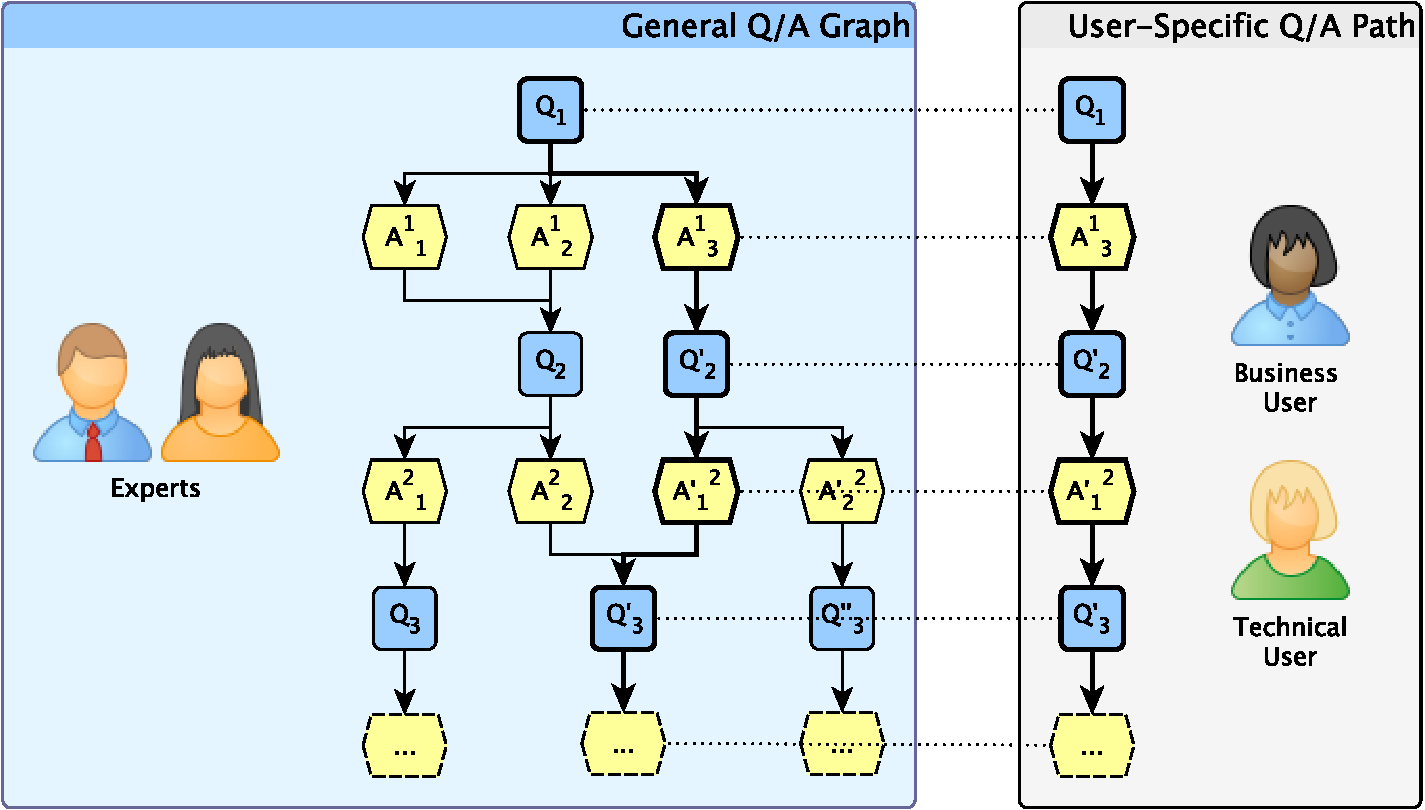
\includegraphics[width=\linewidth]{figures/qa-graph-path.pdf}
    \caption{
        A graphical representation of the \ac{Q/A} mechanism, viewed as a graph by experts and as a sequential path by business and technical users (from~\cite{hicssfairness2025}).
    }
    \label{fig:qa-graph-path}
\end{figure}

The end user can navigate freely through the questionnaire, answering questions and returning to previous ones in case of need.
%
Of course in this way it is possible to change the path, and so the flow of future questions.



% 4. Automation
\section{Automation}

At this stage, it is yet vague how the methodology proposed can inject fairness measures and practical steps into the development process.
%
Here is the point where \acf{TU} contributes to the process, by implementing scripts and computational operations that are eventually integrated into the final system.
%
Said that, \acp{TU} play an important role because, regardless of the complexity and variety of the needed scripts, such scripts can change case by case.
%
Moreover, \ac{TU} is still useful as source of technical knowledge and assistance for the \acf{BU}.

However, while many activities performed by technical users are specific to their respective organizations, certain tasks are generalizable enough to be automated directly by the implemented methodology.
%
Relevant examples of this, are the computation of fairness metrics and the identification of biases in datasets.
%
These, in fact, are enough consolidated to be automated and integrated into the methodology.
%
Rather than requiring individual technical users to develop their own solutions from scratch, the system itself can integrate these capabilities as built-in system-level functions, ensuring consistency, efficiency, and reliability across different projects.

The reification of the meta-methodology should be purposefully designed to facilitate this progression toward greater automation. 
%
When certain actions--—such as evaluating responses or detecting biases--—are widely applicable rather than organization-specific, they can be implemented as reusable system-level solutions.
%
This eliminates redundancy, reducing the need for technical users to repeatedly address the same challenges independently.

These scripts to be injected to the methodology, can be provided by methodology implementation itself, developed by technical users within organizations, or contributed by third-party developers.
%
This flexible approach ensures that automation capabilities can expand over time, adapting to emerging best practices.
%
In the early stages of system adoption, technical users may handle certain tasks manually, but as the methodology matures, these tasks can gradually be automated.

% 4.x in this way we can provide also technical steps
Technically, these scripts can be attached easily to the  software implementation of such methodology, and they can be triggered whenever some kind of events occur, like the answer to a question, or termination of another computation.

% TODO: Strengths and Limitations (pros and cons of the methodology)
% here or at the end?





%----------------------------------------------------------------------------------------
\chapter{Design}%
\label{chap:design}
%----------------------------------------------------------------------------------------

In line with the previous chapter, the objective here is to design a software artifact that reifies the proposed meta-methodology, in order to make it usable by stakeholders to develop fair \ac{AI} systems.
%
Software design must be flexible and adaptable, as the methodology is intended to be subject to changes and improvements over time.

The final product is designed to be used by \acfp{BU} through an intuitive web interface.
%
Hence, frontend will interact with the underlying backend which handles the \ac{Q/A} mechanism and automates technical steps.

\section{Architecture}

\begin{figure}
    \centering
    \includegraphics[width=\linewidth]{figures/diagrams/architecture.png}
    \caption{
        The overall software architecture of the proposed software system.
    }
    \label{fig:architecture}
\end{figure}

The software adopts an \textbf{event-driven} architecture (\cref{fig:architecture}), as events are used to handle part of the communications between the components.
%
This design choice is motivated by the need to trigger automation scripts at specific points, for instance, when a question is answered or when a computation is completed.

The entire system is composed of the following components:
\begin{enumerate}
    \item \textbf{Backend}: the core of the system, managing the \ac{Q/A} mechanism and the automation of technical steps.
    \item \textbf{Database}: a database to store the questions, answers, and other relevant information.
    \item \textbf{Automation Scripts}: a set of pluggable scripts that automate technical steps, such as computing fairness metrics and mitigating biases.
    \item \textbf{Event Broker}: component responsible for event handling in the whole system.
    \item \textbf{Frontend}: the web application that allows \acp{BU} to interact with the system.
\end{enumerate}

\paragraph{Clean Architecture.}

Backend component is the core of the system, it is a web service encapsulating the business logic managing the \ac{Q/A} mechanism.
%
It has been designed using Clean Architecture~\cite{martin2017clean}, in order to separate the business logic from technical details, making the system flexible and technology-agnostic.
%
This means that high-level business logics do not depend on low-level implementation details.
%
And besides, it improves the separation of concerns, separating clearly core concepts, business rules, and technical details.

Therefore, backend is divided into the following layers:

\begin{enumerate}
    \item \textbf{Domain}: the layer containing the core domain entities.
    \item \textbf{Application}: the application-specific business logic.
    \item \textbf{Presentation}: the interface between domain entities and the external technologies.
    \item \textbf{Infrastructure}: the outermost layer, containing the implementation details technology-specific.
\end{enumerate}

% 
The dependency flow is unidirectional, from the outermost layer (Infrastructure) to the innermost one (Domain).
%
So, for instance, Application layer and Presentation layer can depend on Domain layer, but not vice versa.
%

\section{Structure}
% introduce DDD 
%
The design choices considered follow the principles of \textbf{\acf{DDD}}~\cite{millett2015ddd}, a software design philosophy that emphasizes the importance of domain model in the development process.
%
The main goal of \ac{DDD} is to align the software system with the domain model, ensuring that the software reflects the real-world domain as closely as possible.
%
Although the focus of this contribution is not on the software design phase in itself, the adoption of \ac{DDD} is motivated by the volatile nature of the methodology, which is expected to evolve through contributions and improvements from multiple people.

% introduce domain entities

\paragraph{Projects.}
In order to introduce the main \ac{Q/A} entities, it is necessary to define the concept of \texttt{Project}, which is the association with the \ac{AI} system that the \ac{BU} wants to build.
%
In fact, each \texttt{ProjectQuestion} is related to (and also identified by) a specific \texttt{Project}.
%
This is not just a way to distinguish multiple AI systems creations, but also to encode and store project-specific information in a ``store'' called \texttt{ProjectContext} (or only \texttt{Context}).
%
This store is essential because each \ac{AI} system has its own dataset, features, algorithm, and so on.
%
Since these data can be of any nature, and are strongly volatile, the idea is to set up a key-value store, without any kind of constraints, where arbitrary (encoded) information can be stored.
%
For instance, at some point it will be useful to store a key-value pair where the key is the name of the dataset, and the value is the encoded dataset itself.
%
These data then will be available and useful to automation scripts and backend business logic.


\paragraph{\ac{Q/A} mechanism.}

\ac{Q/A} mechanism can be intuitively mapped to two main \textbf{domain entities}: \texttt{Question} and \texttt{Answer}.
%
However, it is necessary to distinguish between questions and answers that are part of the general graph and those that are project-related.
%
Therefore, in the domain model are present the related entities as shown in \cref{fig:entities}.

\begin{figure}
    \centering
    \includegraphics[width=\linewidth]{figures/diagrams/entities.png}
    \caption{
        UML class diagram of main \ac{Q/A} entities.
    }
    \label{fig:entities}
\end{figure}

\texttt{GraphQuestion} represents an extension of the general \texttt{Question} entity, containing a set of answer ids that are meant to ``enable'' such question in the graph.
%
In other words, a \texttt{GraphQuestion} is a question that is part of the general graph, and the set of answer ids is needed to encode the \textit{answer-to-question} edge ($A \to Q$).
%
With regard to admissible answers, for the \texttt{GraphQuestion} is sufficient to rely on the general \texttt{Answer} entity because it doesn't need to have more information.

On the other hand, \texttt{ProjectQuestion}s are part of the project-related graph, and each of them is related to (and also identified by) a specific \texttt{Project}.
%
The main difference between \texttt{GraphQuestion} and \texttt{ProjectQuestion} is that the latter has the possibility to ``select'' a certain answer (in the case of single choice questions) or multiple answers (in the case of multiple choice questions).
%
Indeed, in this case, answers must have a state representing whether they are selected or not.
%
\texttt{ProjectAnswer} entity, in fact, is intended to fulfill this need, as it contains a boolean field, and a \texttt{SelectionStrategy} handling the logics behind the selection.

\vspace{1cm}
\noindent
For each \textbf{domain entity}, other \ac{DDD} building blocks are defined:

\begin{itemize}
    \item \textbf{Factories}: to facilitate the creation of new instances.
    \item \textbf{Repositories}: to manage the persistence of the entities.
    \item \textbf{Services}: to handle the business logic related to the entities.
\end{itemize}

From the structural view point, factories and repositories reside in the Domain layer, as they are intended to simplify the management of domain entities.
%
Services instead, are part of the Application layer, since they compose the entire business logic of the system.
%
However, the persistence of the entities strongly depends on technological details, so, while contracts are defined in the Domain layer, the actual implementations are pushed away to the Infrastructure layer (as shown in \cref{fig:packages}).

\begin{figure}
    \centering
    \includegraphics[width=\linewidth]{figures/diagrams/packages.png}
    \caption{
        Representation of packages structure.
    }
    \label{fig:packages}
\end{figure}

The same applies to the \texttt{EventsService}, which is a particular service handling the event production and consumption.
%
The reason is that an event-driven architecture can be achieved using different technological solutions, and business logic should remain technology-independent.
%
Furthermore, due to this layer organization, it is possible to easily interchange the underlying technologies without affecting business logic and core domain entities (for instance using a relational database instead of a NoSQL one).


\section{Behavior}
\sidenote{to hide backend and automation scripts in tableofcontents?}

The system behavior is mainly concentrated in \textbf{Backend} and \textbf{Automation Scripts} components.

\subsection{Backend}

Backend component is a web service that exposes a REST \ac{API}, enabling clients to interact with questions graph and questionnaires.
%
Its primary functionalities include modifying the question graph structure (adding, removing, modifying questions) and managing project-related questionnaires compilations.
%
It is also possible to create new projects, and, for each of them, starting a new questionnaire session.
%
Summarizing, backend is a simple listening web server, that manages requests and trigger events when relevant actions occur.

However, an important aspect to notice in this component behavior, is the \texttt{Context} update of various projects.
%
\texttt{Context} updates are essential to the correct business logic functioning, because the major part of fairness-related computations strongly depends on the specific data stored in the \texttt{Context}.
%
For example, all data mitigation algorithms require the actual dataset, or the computation of fairness metrics needs the dataset and the selected output and sensitive features.
%
Such computations, can be executed by both backend and automation scripts, for this reason \texttt{Context} updates represent a key point in the system behavior.

\subsection{Automation Scripts}

Automation Scripts are responsible for responding to specific domain events, performing necessary (fairness-related) computations, and updating system state.
%
These scripts act as event-driven processes that listen for predefined triggers, such as selecting an answer to a question, creation of a new dataset, or completion of a fairness metric computation.
%
Once the processing is completed, they send relevant updates back to the backend via \ac{API} requests, ensuring that the system remains up-to-date and operates seamlessly without requiring manual intervention.

\section{Interaction}
The starting point of interactions is \ac{BU} that interacts with the system through the Frontend component.
%
Frontend is in charge of presenting questions to the \ac{BU}, collecting answers, and sending them to the backend service.
%
The backend, in turn, processes the requests and updates the questionnaire state accordingly.
%
At this point, backend service triggers an event for each relevant action undertaken, which is caught by all Automation Scripts previously subscribed to the Broker.
%
Each script performs its computation, and eventually sends back the results to the backend, which updates the system state and notifies the frontend to display the results (if there are any) to the \ac{BU}.
%
It is also possible that, during computations, are triggered other events for other relevant actions, like the processing of a new dataset.

The entire interaction flow is shown in \cref{fig:sequence}.

\begin{figure}
    \centering
    \includegraphics[width=0.70\linewidth]{figures/diagrams/sequence.png}
    \caption{
        Generic sequence diagram showing the interactions between main components.
    }
    \label{fig:sequence}
\end{figure}



\section{\acs{API}}

\subsection{Rest}

Backend service exposes an \ac{API} used to interact with the three main entities: \textbf{projects}, \textbf{questions} graph, and \textbf{questionnaires}.
%
Resources are organized following the REST principles, and each resource is identified by a unique URI.
%
Since questionnaires are project-related, such resource is under the \texttt{Project} hierarchy.
%
In \cref{fig:rest-api} are shown the main endpoints of the \ac{API}.


\begin{figure}
    \centering
    \subfloat[\ac{API} for \texttt{Question} operations]{%
        \includegraphics[width=0.32\textwidth]{figures/api/api-questions.png}
    }
    \hfill
    \subfloat[\ac{API} for \texttt{Project} operations]{%
        \includegraphics[width=0.32\textwidth]{figures/api/api-projects.png}
    }
    \hfill
    \subfloat[\ac{API} for \texttt{Questionnaire} operations]{%
        \includegraphics[width=0.32\textwidth]{figures/api/api-questionnaires.png}
    }
    
    \caption{Backend REST \ac{API} endpoints.}
    \label{fig:rest-api}
\end{figure}


\subsection{Events}

The other method available to interact with the system, which powers also internal communications, is the event-driven one.
%
This represents an \ac{API} slightly different from the classic REST one. 
%
Here, \ac{API} endpoints are channels on which operations of type \texttt{send} and \texttt{receive} are performed.
%
This type of \ac{API} enables asynchronous communication between system components, in this case, the backend and automation scripts.
%
That's fundamental because computations are intended to be non-blocking in order to allow \ac{BU} to proceed in the questionnaire compilation.

\begin{figure}
    \centering
    \subfloat[Publish operation for a channel]{%
        \includegraphics[width=0.48\textwidth]{figures/api/async-api-send.png}
    }
    \hfill
    \subfloat[Receive operation for a channel]{%
        \includegraphics[width=0.48\textwidth]{figures/api/async-api-receive.png}
    }
    
    \caption{Async \ac{API} channels example.}%
    \label{fig:async-api}
\end{figure}

A documentation example of such \ac{API} is shown in \cref{fig:async-api} using Async \ac{API} specification (\href{https://www.asyncapi.com}{https://www.asyncapi.com}). The main concepts in this are:

\begin{itemize}
    \item \textbf{Channels}: Specific topics where events are published. Each topic corresponds to a particular type of event.
    \item \textbf{Operations}: Primarily \texttt{send} (\texttt{publish}), to publish events on the channel, and \texttt{receive} (performing if \texttt{subscribed} to channel), to receive messages when events are published.
    \item \textbf{Messages}: Schemas of the objects published on channels.
\end{itemize}


This API is highly flexible, in fact, when an automation script is created, it can be attached to a new channel created ad hoc for the script specific purpose.
%
For instance, a new script can be plugged in simply  creating a new channel and subscribing at it.




%----------------------------------------------------------------------------------------
\chapter{Implementation}%
\label{chap:implementation}
%----------------------------------------------------------------------------------------

This chapter delves into the technical details of the software implementation which reifies the proposed meta-methodology.
%
It provides an overview of the deployed architecture, and, basing on the design choices made in the previous chapter, it explains how the various components are actually implemented.
% 
The chapter also covers the deployment phase of the software system, how to set up the configuration environment, and in the end how to run it.
%
Finally, the chapter concludes covering some use cases to demonstrate the system in action, providing also \acf{BU} perspective through the web interface.


\section{Components}


\paragraph{Backend.}

% 1. explaining why backend web service in python (reduce abstraction gap)

Backend component is implemented as a web service in Python. The choice aims to reduce the abstraction gap because python comes with consolidated frameworks that facilitate development of \ac{AI} systems.
%
Python represents also a good choice thanks to its readability and simplicity, which make it easier to be maintained and extended by developers who were not originally involved in the project.
%
\href{https://flask-restful.readthedocs.io/en/latest/}{Flask-restful} framework has been used to ease the development of the web service, as it allows the creation of a RESTful \ac{API} with few lines of code (\cref{lst:api-code}).


\lstinputlisting[float,language=Python,label={lst:api-code},caption={Example resource creation with Flask-restful.}]{listings/api.py}


\paragraph{Event Broker.}

% 2. explaining why kafka (event-driven architecture)
\href{https://kafka.apache.org/}{Apache Kafka} is used as the event broker to implement the event-driven architecture.
%
Kafka is a distributed streaming platform that provides high throughput, scalability, and fault tolerance.
%
The python client of Kafka has been used to interact with the broker, allowing the backend and automation scripts to publish and subscribe to events.
%
This is achieved by an ad hoc service implemented in the infrastructure layer (\cref{lst:kafka-python}).

\lstinputlisting[float,language=Python,label={lst:kafka-python},caption={Example resource creation with Flask-restful.}]{listings/kafka.py}


\paragraph{Database.}

% 3. talking about the graph database (neo4j) and why it fits well with the graph structure of the Q/A mechanism
For the database, the choice fell on graph database, as it fits well with the graph structure of the \ac{Q/A} mechanism, and the technical implementation chosen is \href{https://neo4j.com/}{Neo4j}.
%
It allows for efficient traversal and querying of the graph, making it easier to manage operations on questions and answers.

% 3.1 how are mapped entities to the database?
Entities are mapped to the database as nodes and relationships.
%
In particular, \textbf{question graph} is mapped as the following: questions and answers are represented as nodes, while the edges between them are represented as relationships.
%
More precisely, let's consider $Q_G$ is the node representation of question $Q$ and $A_G$ is the node representation of answer $A$ (both in general graph).
%
Edges in Neo4j are associated with a label, so edges of type $Q \to A$ are stored as $Q_G \xrightarrow{\text{HAS\_ANSWER}} A_G$, while edges of type $A \to Q$ are actually stored as $A_G \xrightarrow{\text{ENABLED\_BY}} Q_G$.


% 3.2 talking about the context (storing key-values in the project node)
With respect to the \texttt{Project}, let's consider $P$ as the node representation of project.
%
Key-value pairs of its \texttt{Context} are stored in $P$.
%
This is straightforward because each node in Neo4j can store arbitrary key-value pairs, making it easy and flexible to save context data.
%
In order to save space, context data that are common to all projects are stored in a separate node named \texttt{PublicContext}, which is referred if a key is not found in the specific project node on which the context data is requested.

Eventually, each \textbf{questionnaire} (if exists) is linked to a specific project $P$ through a relationship $P \xrightarrow{\text{QUESTIONNAIRE}} Q_P$, where $Q_P$ is the root of the questionnaire graph (the first question asked), and it is created upon the root of the general graph.
%
Next questions in the questionnaire path are linked to the previous ones through relationships of kind $Q'_P \xrightarrow{\text{NEXT}} Q''_P$.

To keep track of the answers given by the \ac{BU}, each answer is linked to the corresponding question through a relationship $Q_P \xrightarrow{\text{HES\_SELECTED}} A_P$, where $A_P$ is the node representation of the answer given by the \ac{BU}.

\paragraph{Automation Scripts.}

% 4 they just need to adhere to the async api (event-driven architecture)
Automation scripts are processes created ad hoc to perform specific computations.
%
They just need to adhere to the Async API specification to be seamless integrated into the system.
%
% By following the Async API, scripts can subscribe to relevant events, perform the necessary computations, and send updates back to the backend, ensuring a smooth and efficient workflow.

% 4.1 about automation script, actually they can be implemented in any language, (python is still the best choice since computations are about ML models and fairness metrics)
These scripts can actually be implemented in any language, but the ones implemented so far are created in Python.
%
One motivation is that in this way scripts can share the backend code benefiting from reusability.
Python is also recommended due to its extensive support for machine learning libraries and frameworks.



\paragraph{Frontend.}

% 5 about frontend, it is a Single Page Application interacting with the backend, implemented using React/Next.js (component base to exploit reusability)
Frontend is implemented as a Single Page Application (SPA) using \href{https://react.dev/}{React} and \href{https://nextjs.org/}{Next.js}.
%
This choice leverages the component-based architecture of React, which promotes reusability and maintainability of the code.
%
Next.js enhances the development experience by providing server-side rendering and static site generation.
%
The component-based architecture fits well because the questionnaire can evolve, and the frontend must be arranged to be changed accordingly.
%
A web-based technology has been chosen for several reasons:
\begin{enumerate*}[label=(\roman*)]
    \item cross-platform compatibility,
    \item ease deployment and maintenance,
    \item accessibility,
    \item powerful features offered by modern frameworks.
\end{enumerate*}



% TODO: needs to be referenced
\begin{figure}
    \centering
    \includegraphics[width=\linewidth]{figures/diagrams/deployment.png}
    \caption{
        Deployment diagram of the system.
    }
    \label{fig:deployment}
\end{figure}

\section{Testing}



%----------------------------------------------------------------------------------------
\chapter{Validation}%
\label{chap:validation}
%----------------------------------------------------------------------------------------

\section{Meta-Methodology Requirements}

\begin{itemize}[label={}]

    \item \textbf{\ref{req:R1}---Requirements Translation} $\rightarrow$ \textbf{\ac{Q/A} Mechanism}:
    %
    the methodology involves socio-legal requirements translation into a simple and structured set of questions. 
    %
    A set of question designed for non-techcnical and non-legal people are more comprehensive than a set of legal constraints.
    %
    Through this mechanism, it is also possible to practically constrain the development process depending on the paths designed in the question graph.

    \item \textbf{\ref{req:R2}---Context and Domain Awareness} $\rightarrow$ \textbf{Questions Design}:
    %
    through a well-designed set of questions, it is possible to incrementally collect information about the application domain and the cultural context in which the system operates.
    %
    Depending on the answers given by the \ac{BU}, the system can adapt the flow of questions branching at the right points, providing tailored questions based on the context.
    
    For instance, answers at the question ``In which area of application will the system be used?'' will influence the following questions, leading to a questionnaire customization based on the application domain.

    \item \textbf{\ref{req:R3}---Adaptability} $\rightarrow$ \textbf{Questions Graph}:
    %
    adaptability is intrinsically achieved by using a graph structure to represent the \ac{Q/A} mechanism.
    %
    In fact, it is possible to change the graph structure easily, adding, removing, or modifying questions and answers, creating new paths, and so on.
    %
    This also enables a ``versioning'' mechanism, which effectively addresses a possible volatile context.
    
    \item \textbf{\ref{req:R4}---Legacy and Novel Systems} $\rightarrow$ \textbf{Adaptability}:
    %
    achieving adaptability(\ref{req:R3}), the methodology can support different situations: it is possible to design a path for creating a new system, as well as a path for an existing one.
    %
    % TODO: to reason about

    
    \item \textbf{\ref{req:R5}---Building the AI System} $\rightarrow$ \textbf{Software Reification}:
    %
    this contribution, rather than providing just an abstract specification of the methodology, provides also a guideline-provisioning software system usable directly by stakeholders.
    %
    In the workflow, \ac{BU} interacting with the system, can compile the questionnaire but at the same time, behind the scenes, backend processes operate to automate technical steps such as training and mitigation.
    %
    In the end, the system will provide an \ac{AI} system that has been subject to fairness considerations since the beginning of the development process.
\end{itemize}



\section{Software Implementation}
% 2. Validation of the software implementation


\section{Limitations}

% Requirement 1 limitation -> the methodology is not providing a methodological way to translate requirements into questions, this phase still needs a collaborative design
With respect to the satisfaction of~\ref{req:R1}, it is defined \textit{what} translated socio-legal requirements should be, but not exactly \textit{how} to translate them.
%
This still represents a complex collaborative challenge by a multidisciplinary team of experts, and it is not automatically addressed by the methodology.
%
However, the methodology simplifies the process by providing itself some constraints.
%
In other words, it forces the subjects involved in the requirements engineering to think about laws and legal constraints in a pragmatic way, in order to translate them into a set of questions that can be answered by a person with no expertise.


% Requirement 3 limitation on "versioning" 
\sidenote{qua spiego bene il versioning, forse va messo da un altra parte?}
Flexibility of question graph, which satisfies \ref{req:R3}, enables a \textit{versioning} mechanism because changing the graph structure means creating a ``new version'' of the methodology.
%
New version means a graph with different paths of questions and answers, which obviously, addresses diverse needs.
%
Hence, the methodology can adapt to evolvable cultural contexts, creating new graphs for each needed change in the application domain.

Conversely, questionnaires already started or completed, are affected by a version change.
%
The reason is due to the strong dependency between questionnaire (project-related graph) and general question graph.
%
In fact, each update to the questionnaire relies on the general graph, and so, general graph changes will lead to inconsistencies in the questionnaire.
%
So, in case of a version change, it is necessary to keep the oldest version to not break the support for the already started questionnaires.
%
At the moment, the only way to adapt to new versions, is to start a new project (and relative questionnaire) from scratch.



% limitations on AI system building
A possible limitation respect to~\ref{req:R5}, is regarding the variety of \ac{AI} systems that can be built.
%
Indeed, software allows uploading datasets of any dimensions, and this could lead to possible issues in terms of computational resources.
%
Theoretically, the methodology does not impose any constraint on the size of dataset or the complexity of the model, but in practice (using the software provided), it is necessary to consider the computational power available to the system.

% long training
Another important aspect is the time needed to perform fairness computations and model training, which can be a bottleneck in the system.
%
This problem not only influences the backend system, but also affects the user experience, as the \ac{BU} has to wait for the system to proceed correctly the questionnaire.
%
Actually, computations performed by backend service and automation scripts are designed to be asynchronous to improves the user experience, but with the assumption that eventually, in a reasonable time, computations will terminate and user will be able to proceed with updated information.
%
If computations take too long, \ac{BU} could proceed with missing or outdated information, leading to possible misuses of the system.


\section{Usage Example}


%----------------------------------------------------------------------------------------
\chapter{Conclusions}%
\label{chap:conclusions}
%----------------------------------------------------------------------------------------



%----------------------------------------------------------------------------------------
% BIBLIOGRAPHY
%----------------------------------------------------------------------------------------

\backmatter

% \nocite{*} % Remove this as soon as you have the first citation

\bibliographystyle{alpha}
\bibliography{bibliography}

\begin{acknowledgements} % this is optional
Optional. Max 1 page.
\end{acknowledgements}

\end{document}
